\documentclass[11pt,a4paper]{article}

\usepackage[a4paper,margin=2.25cm]{geometry}
\usepackage[T1]{fontenc}
\usepackage[utf8]{inputenc}
\usepackage{lmodern}
\usepackage{microtype}
\usepackage{amsmath,amssymb,mathtools,bm}
\usepackage{booktabs,longtable,array,tabularx,multirow}
\usepackage{graphicx}
\usepackage{xcolor}
\usepackage{enumitem}
\usepackage{tcolorbox}
\tcbuselibrary{breakable,skins}
\usepackage{tikz}
\usetikzlibrary{arrows.meta,positioning,calc,fit}
\usepackage{caption}
\usepackage{subcaption}
\usepackage{hyperref}
\usepackage[nameinlink,capitalise]{cleveref}
\usepackage{fancyhdr}
\usepackage{titlesec}
\usepackage{setspace}
\usepackage{bm}
\usepackage{siunitx}
\usepackage{float}

\definecolor{deepblue}{RGB}{27,76,128}
\definecolor{softblue}{RGB}{238,245,252}
\definecolor{deepgreen}{RGB}{39,111,79}
\definecolor{softgreen}{RGB}{239,249,243}
\definecolor{deeporange}{RGB}{180,91,31}
\definecolor{softorange}{RGB}{253,246,238}
\definecolor{deepred}{RGB}{154,45,45}
\definecolor{softgray}{RGB}{247,247,247}

\hypersetup{
  colorlinks=true,
  linkcolor=deepblue,
  citecolor=deepgreen,
  urlcolor=deepblue,
  pdftitle={Controlled q-Voter Theory for Round-Level Feedback: A Step-by-Step Tutorial},
  pdfauthor={Tutorial report}
}

\pagestyle{fancy}
\fancyhf{}
\fancyhead[L]{Controlled $q$-Voter Theory Tutorial}
\fancyhead[R]{Round-Level Feedback and Transfer Entropy}
\fancyfoot[C]{\thepage}
\setlength{\headheight}{14pt}

\titleformat{\section}{\Large\bfseries\color{deepblue}}{\thesection}{0.8em}{}
\titleformat{\subsection}{\large\bfseries\color{deepblue}}{\thesubsection}{0.7em}{}
\titleformat{\subsubsection}{\normalsize\bfseries\color{deepgreen}}{\thesubsubsection}{0.6em}{}

\newtcolorbox{intuitionbox}[1][]{
  breakable,
  colback=softblue,
  colframe=deepblue,
  boxrule=0.7pt,
  arc=2mm,
  title=Intuition,
  fonttitle=\bfseries,
  #1
}
\newtcolorbox{logicbox}[1][]{
  breakable,
  colback=softgreen,
  colframe=deepgreen,
  boxrule=0.7pt,
  arc=2mm,
  title=Logic of the step,
  fonttitle=\bfseries,
  #1
}
\newtcolorbox{warningbox}[1][]{
  breakable,
  colback=softorange,
  colframe=deeporange,
  boxrule=0.7pt,
  arc=2mm,
  title=Common point of confusion,
  fonttitle=\bfseries,
  #1
}
\newtcolorbox{resultbox}[1][]{
  breakable,
  colback=softgray,
  colframe=black!55,
  boxrule=0.8pt,
  arc=1.5mm,
  title=Result,
  fonttitle=\bfseries,
  #1
}

\newcommand{\Adv}{\ensuremath{\mathrm{Advocate}}}
\newcommand{\NoOp}{\ensuremath{\mathrm{NoOp}}}
\newcommand{\KL}{D_{\mathrm{KL}}}
\newcommand{\JS}{\mathrm{JS}}
\newcommand{\Prb}{\operatorname{Pr}}
\newcommand{\E}{\mathbb{E}}
\newcommand{\Var}{\operatorname{Var}}
\newcommand{\1}{\mathbbm{1}}

\setlength{\parindent}{0pt}
\setlength{\parskip}{0.55em}
\onehalfspacing

\begin{document}

\begin{titlepage}
\centering
\vspace*{2.2cm}
{\Huge\bfseries Controlled $q$-Voter Theory for Round-Level Feedback\par}
\vspace{0.4cm}
{\LARGE A Step-by-Step Tutorial on the Calculations Behind the Exact and Mean-Field Transfer-Entropy Results\par}
\vspace{1.4cm}
{\large Based on the five-page theory note dated 14 August 2026\par}
\vspace{1.0cm}
\begin{tcolorbox}[width=0.84\textwidth,colback=softblue,colframe=deepblue,arc=2mm]
\centering
\textbf{Purpose.} This document is intentionally pedagogical. Every symbol is defined, the probability calculations are unpacked, algebraic simplifications are shown explicitly, and the logic of each construction is explained before the formal result is used.
\end{tcolorbox}
\vfill
{\large 20 August 2026\par}
\end{titlepage}

\begin{abstract}
This tutorial derives, step by step, the controlled unanimity $q$-voter model with round-level feedback and the transfer-entropy quantities reported in the source theory note. The population consists of $N$ binary agents. At the start of each round, a controller samples $q_c$ agents, chooses either \NoOp{} or \Adv{} through a soft sigmoid policy, and, if it advocates target opinion $A$, replaces one of the $q$ social-input slots at exactly $b$ of the $N$ microscopic update positions. We first derive the ordinary and controlled one-update kernels $K_0$ and $K_1$, then construct the exact whole-round kernels $R_0$ and $R_1$, including the dynamic-programming recursion that averages exactly over all uniformly preallocated control schedules. We then derive the exact finite-$N$ local transfer entropy $T(n)=I(U_k;N_{k+1}\mid N_k=n)$ and show why it is a weighted Jensen--Shannon divergence. Finally, we derive the large-$N$, weak-control approximation and the analytically stronger $q=1$ special case, explaining the $c^2$ control-budget scaling and the boundary distinction $q=1:T(0)>0$ versus $q\ge2:T(0)=0$. Reproduced theory curves are included to connect every expression to the reported results.
\end{abstract}

\tableofcontents
\newpage

\section{What problem are we solving?}

We study a population of $N$ agents. Every agent currently supports one of two opinions,
\[
A \qquad \text{or} \qquad B.
\]
The population evolves through a unanimity $q$-voter rule: a focal agent switches only when all $q$ social inputs unanimously support the opposite opinion.

An external controller tries to favor opinion $A$. The controller does not directly overwrite the focal agent's decision rule. Instead, it can insert one pro-$A$ social input into selected microscopic updates. Its action is chosen only once per population round after observing a finite sample of the population.

The central information-theoretic question is
\begin{equation}
I(U_k;N_{k+1}\mid N_k),
\label{eq:central_te}
\end{equation}
where $U_k$ is the controller's round-level action, $N_k$ is the number of $A$ supporters at the beginning of round $k$, and $N_{k+1}$ is the number at the beginning of the next round.

\begin{intuitionbox}
Conditioning on $N_k$ asks a very precise causal-predictive question: \emph{if we compare rounds that start from the same population count, does learning whether the controller advocated or did nothing improve our prediction of the next population count?}
\end{intuitionbox}

The calculation proceeds through four layers:
\[
\boxed{\text{microscopic population rule}}
\Longrightarrow
\boxed{K_0,K_1}
\Longrightarrow
\boxed{R_0,R_1}
\Longrightarrow
\boxed{T(n)}.
\]
The rest of this tutorial builds these objects one at a time.

\section{State, timing, variables, and parameters}

\subsection{Population state}

At the start of round $k$, let
\begin{equation}
N_k=n\in\{0,1,\ldots,N\}.
\end{equation}
Thus $n$ agents support $A$, and
\[
N-n
\]
agents support $B$.

It is often convenient to use the corresponding fraction
\begin{equation}
x_k=\frac{N_k}{N},\qquad x=\frac{n}{N}\in[0,1].
\end{equation}
Interpretation:
\[
x=0 \Rightarrow \text{all }B,\qquad
x=\frac12 \Rightarrow \text{even split},\qquad
x=1 \Rightarrow \text{all }A.
\]

\subsection{Symbol table}

\begin{longtable}{>{\raggedright\arraybackslash}p{2.0cm}>{\raggedright\arraybackslash}p{11.8cm}}
\toprule
\textbf{Symbol} & \textbf{Meaning} \\
\midrule
\endfirsthead
\toprule
\textbf{Symbol} & \textbf{Meaning} \\
\midrule
\endhead
$N$ & Population size. One population round contains exactly $N$ microscopic focal-update positions. \\
$q$ & Number of social inputs used by the unanimity $q$-voter response rule. \\
$q_c$ & Number of agents sampled by the controller at the beginning of a round. This is a sensing resource, not the social-interaction order. \\
$b$ & Exact number of microscopic update positions controlled during an advocacy round. \\
$c=b/N$ & Fraction of microscopic positions controlled during an advocacy round. \\
$N_k$ & Number of $A$ supporters at the start of round $k$. \\
$n$ & A particular value of $N_k$. \\
$x=n/N$ & Fraction of $A$ supporters corresponding to state $n$. \\
$Y_k$ & Number of $A$ supporters observed in the controller's sample. \\
$y$ & A particular value of $Y_k$, with $0\le y\le q_c$. \\
$U_k$ & Controller action during round $k$: $\NoOp$ or $\Adv$. \\
$\theta$ & Intervention threshold in the controller's sigmoid policy. \\
$\beta$ & Slope / decision stochasticity of the controller policy. Large $\beta$ makes the policy more threshold-like. \\
$K_0$ & One-microscopic-update transition kernel without controller advocacy. \\
$K_1$ & One-microscopic-update transition kernel at a controlled position, where one social slot is replaced by a controller message supporting $A$. \\
$R_0$ & Whole-round transition kernel under $\NoOp$. \\
$R_1$ & Whole-round transition kernel under $\Adv$. \\
$S(y\mid n)$ & Sensor law: probability that the controller sees $y$ target supporters when the true population count is $n$. \\
$a_n$ & State-conditioned advocacy probability $\Prb(U_k=\Adv\mid N_k=n)$. \\
$M_n(m)$ & Next-state distribution after marginalizing over the controller action. \\
$T(n)$ & Exact state-local transfer entropy $I(U_k;N_{k+1}\mid N_k=n)$. \\
$P_k(n)$ & Distribution of the population count at the start of round $k$. \\
$T_k$ & Round-$k$ transfer entropy $I(U_k;N_{k+1}\mid N_k)$. \\
$T^{(K)}$ & Average transfer entropy over a finite $K$-round episode. \\
$f_0(x)$ & Large-$N$ ordinary microscopic drift in the count variable. \\
$f_1(x)$ & Large-$N$ controlled microscopic drift. \\
$\Delta f_q(x)$ & Drift separation $f_1(x)-f_0(x)$. \\
$\nu_0(x)$ & Ordinary microscopic variance coefficient. \\
\bottomrule
\end{longtable}

\subsection{Round timing}

The timing is
\begin{center}
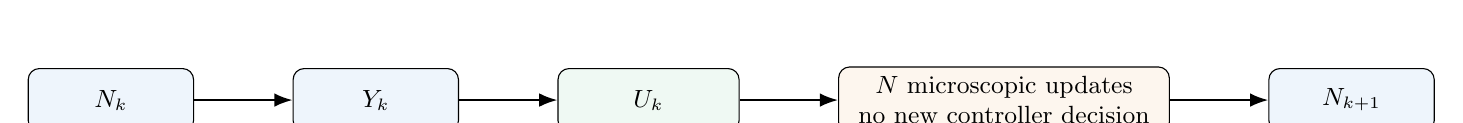
\begin{tikzpicture}[node distance=1.25cm,>=Latex, every node/.style={font=\small}]
\node[draw,rounded corners,fill=softblue,minimum width=2.1cm,minimum height=.8cm] (N) {$N_k$};
\node[draw,rounded corners,fill=softblue,right=of N,minimum width=2.1cm,minimum height=.8cm] (Y) {$Y_k$};
\node[draw,rounded corners,fill=softgreen,right=of Y,minimum width=2.3cm,minimum height=.8cm] (U) {$U_k$};
\node[draw,rounded corners,fill=softorange,right=of U,minimum width=4.2cm,minimum height=.8cm,align=center] (micro) {$N$ microscopic updates\\no new controller decision};
\node[draw,rounded corners,fill=softblue,right=of micro,minimum width=2.1cm,minimum height=.8cm] (Nnext) {$N_{k+1}$};
\draw[->,thick] (N)--(Y);
\draw[->,thick] (Y)--(U);
\draw[->,thick] (U)--(micro);
\draw[->,thick] (micro)--(Nnext);
\end{tikzpicture}
\end{center}

If $U_k=\Adv$, a set
\[
S_k\subset\{1,\ldots,N\},\qquad |S_k|=b,
\]
of microscopic \emph{positions} is drawn uniformly before the round. The controller does not select $b$ fixed agent identities. This keeps the dynamics exchangeable at the population level.

\begin{warningbox}
The controller acts \emph{once per round}, not once per microscopic update. The $N$ microscopic positions use the already-chosen round action. This is why the natural information channel is from $U_k$ to $N_{k+1}$ conditional on $N_k$.
\end{warningbox}

\section{Ordinary microscopic $q$-voter kernel $K_0$}

A single microscopic update changes the number of $A$ supporters by at most one:
\[
n\longrightarrow n+1,\qquad n\longrightarrow n,\qquad n\longrightarrow n-1.
\]
We derive all three probabilities.

\subsection{Derivation of $K_0(n+1\mid n)$}

For $n$ to increase by one, a $B$ agent must switch to $A$. Two independent selection requirements must both occur.

\subsubsection{Requirement 1: the focal agent is a $B$ supporter}

There are $N-n$ such agents among $N$ total agents, so
\begin{equation}
\Prb(\text{focal is }B\mid n)=\frac{N-n}{N}.
\label{eq:focalB}
\end{equation}

\subsubsection{Requirement 2: all $q$ sampled social inputs are $A$ supporters}

After the focal agent is removed, there are $N-1$ possible neighbors. Because the focal agent is $B$, all $n$ existing $A$ supporters remain available among these $N-1$ agents.

The total number of unordered groups of $q$ neighbors is
\[
\binom{N-1}{q}.
\]
The number of groups consisting entirely of $A$ supporters is
\[
\binom{n}{q}.
\]
Therefore
\begin{equation}
\Prb(\text{all }q\text{ inputs are }A\mid \text{focal }B,n)
=
\frac{\binom{n}{q}}{\binom{N-1}{q}}.
\label{eq:allA}
\end{equation}

\subsubsection{Multiply the two requirements}

Using \cref{eq:focalB,eq:allA},
\begin{align}
K_0(n+1\mid n)
&=
\underbrace{\frac{N-n}{N}}_{\color{deepblue}{\text{choose focal }B}}
\underbrace{\frac{\binom{n}{q}}{\binom{N-1}{q}}}_{\color{deepgreen}{\text{all }q\text{ inputs are }A}}.
\end{align}
Hence
\begin{resultbox}
\begin{equation}
\boxed{
K_0(n+1\mid n)
=
\frac{N-n}{N}
\frac{\binom{n}{q}}{\binom{N-1}{q}}.}
\label{eq:k0plus}
\end{equation}
\end{resultbox}

\subsection{Derivation of $K_0(n-1\mid n)$}

Now an $A$ supporter must switch to $B$.

The focal agent is $A$ with probability
\[
\frac{n}{N}.
\]
If the focal agent is $A$, the other $N-1$ agents contain all $N-n$ $B$ supporters. Unanimous $B$ input occurs with probability
\[
\frac{\binom{N-n}{q}}{\binom{N-1}{q}}.
\]
Thus
\begin{resultbox}
\begin{equation}
\boxed{
K_0(n-1\mid n)
=
\frac{n}{N}
\frac{\binom{N-n}{q}}{\binom{N-1}{q}}.}
\label{eq:k0minus}
\end{equation}
\end{resultbox}

\subsection{The diagonal probability}

The three possibilities exhaust all outcomes, so the row must sum to one:
\begin{equation}
\boxed{
K_0(n\mid n)
=1-K_0(n+1\mid n)-K_0(n-1\mid n).}
\label{eq:k0diag}
\end{equation}
This completes the ordinary microscopic kernel.

\section{Controlled microscopic kernel $K_1$}

At a controlled position, the focal response rule remains a unanimity $q$-voter rule. The only change is that one of the $q$ social-input slots is occupied by a controller message supporting $A$.

Thus the focal agent sees
\[
\boxed{1\text{ controller input saying }A+(q-1)\text{ ordinary inputs}.}
\]

\subsection{Derivation of $K_1(n+1\mid n)$}

As before, the focal agent must be a $B$ supporter, giving
\[
\frac{N-n}{N}.
\]
But one required $A$ input has already been supplied by the controller. Only $q-1$ ordinary $A$ supporters are now required:
\[
\frac{\binom{n}{q-1}}{\binom{N-1}{q-1}}.
\]
Therefore
\begin{resultbox}
\begin{equation}
\boxed{
K_1(n+1\mid n)
=
\frac{N-n}{N}
\frac{\binom{n}{q-1}}{\binom{N-1}{q-1}}.}
\label{eq:k1plus}
\end{equation}
\end{resultbox}

\subsection{Why $K_1(n-1\mid n)=0$}

For an $A$ focal agent to switch to $B$, all $q$ inputs must be $B$. But one slot is fixed to the controller's $A$ message. Unanimous $B$ input is therefore impossible:
\begin{resultbox}
\begin{equation}
\boxed{K_1(n-1\mid n)=0.}
\label{eq:k1minus}
\end{equation}
\end{resultbox}
The diagonal term is
\begin{equation}
\boxed{K_1(n\mid n)=1-K_1(n+1\mid n).}
\end{equation}

\begin{intuitionbox}
Control works in two ways simultaneously: it makes $B\to A$ easier because only $q-1$ ordinary $A$ inputs are needed, and it blocks $A\to B$ at controlled positions because the controller's $A$ message prevents unanimous $B$ input.
\end{intuitionbox}

\section{Worked microscopic example: $N=32$, $q=2$, $n=8$}

This example makes the abstract kernels concrete.

We have
\[
N=32,\qquad q=2,\qquad n=8,\qquad x=\frac{8}{32}=0.25.
\]
There are $24$ $B$ supporters.

\subsection{Ordinary increase probability}

From \cref{eq:k0plus},
\begin{align}
K_0(9\mid8)
&=\frac{24}{32}\frac{\binom82}{\binom{31}{2}}\\
&=\frac34\frac{28}{465}\\
&\approx 0.04516.
\end{align}

\subsection{Ordinary decrease probability}

From \cref{eq:k0minus},
\begin{align}
K_0(7\mid8)
&=\frac8{32}\frac{\binom{24}{2}}{\binom{31}{2}}\\
&=\frac14\frac{276}{465}\\
&\approx 0.14839.
\end{align}
So the uncontrolled microscopic dynamics at this state favor movement toward $B$.

\subsection{Controlled increase probability}

For $q=2$, a controlled position needs only $q-1=1$ ordinary $A$ supporter:
\begin{align}
K_1(9\mid8)
&=\frac{24}{32}\frac{\binom81}{\binom{31}{1}}\\
&=\frac34\frac8{31}\\
&=\frac6{31}\\
&\approx 0.19355.
\end{align}
Meanwhile,
\[
K_1(7\mid8)=0.
\]

\begin{logicbox}
The controlled input changes the one-step process from roughly
\[
P(+1)=0.045,\qquad P(-1)=0.148
\]
to
\[
P(+1)=0.194,\qquad P(-1)=0.
\]
The whole-round theory simply propagates these microscopic differences through $N$ sequential update positions.
\end{logicbox}

\section{Controller sensing: the hypergeometric law}

The controller does not observe $n$ directly. At the start of the round it samples $q_c$ agents without replacement and records
\[
Y_k=y,
\]
the number of sampled agents supporting $A$.

We derive
\[
S(y\mid n)=\Prb(Y_k=y\mid N_k=n).
\]
To obtain exactly $y$ sampled $A$ supporters:
\begin{itemize}[leftmargin=1.5em]
\item choose $y$ agents from the $n$ available $A$ supporters: $\binom{n}{y}$ possibilities;
\item choose the remaining $q_c-y$ agents from the $N-n$ $B$ supporters: $\binom{N-n}{q_c-y}$ possibilities;
\item divide by the number of all possible samples of size $q_c$: $\binom{N}{q_c}$.
\end{itemize}
Therefore
\begin{resultbox}
\begin{equation}
\boxed{
S(y\mid n)
=
\Prb(Y_k=y\mid N_k=n)
=
\frac{\binom{n}{y}\binom{N-n}{q_c-y}}{\binom{N}{q_c}}.}
\label{eq:sensor}
\end{equation}
\end{resultbox}

\begin{warningbox}
$q$ and $q_c$ are different parameters. $q$ belongs to the population's social response rule. $q_c$ belongs only to the controller's measurement process.
\end{warningbox}

\section{The soft round controller}

Given sensor outcome $y$, the measured target fraction is
\[
\frac{y}{q_c}.
\]
The controller uses the sigmoid policy
\begin{equation}
\Prb(U_k=\Adv\mid Y_k=y)
=
\sigma\!\left[\beta\left(\theta-\frac{y}{q_c}\right)\right],
\qquad
\sigma(z)=\frac{1}{1+e^{-z}}.
\label{eq:softpolicy}
\end{equation}

\subsection{What do $\theta$ and $\beta$ do?}

$\theta$ is the intervention trigger. With $\theta=1/2$, advocacy becomes more likely when the measured target fraction is below one half.

$\beta$ controls how sharply the controller responds to the threshold:
\[
\beta\to0 \Rightarrow \sigma(\beta\cdot)\approx\frac12,
\]
so the decision is nearly random, whereas large $\beta$ makes the policy close to a deterministic threshold rule.

\subsection{Average over sensor uncertainty}

We need the advocacy probability conditioned on the \emph{true} state $n$:
\[
a_n\equiv\Prb(U_k=\Adv\mid N_k=n).
\]
The controller does not see $n$, so we marginalize over all possible $y$:
\begin{align}
a_n
&=\sum_y
\Prb(Y_k=y\mid n)
\Prb(\Adv\mid Y_k=y)\\
&=\sum_y
S(y\mid n)
\sigma\!\left[\beta\left(\theta-\frac{y}{q_c}\right)\right].
\end{align}
Thus
\begin{resultbox}
\begin{equation}
\boxed{
a_n
=
\sum_y
S(y\mid n)
\sigma\!\left[\beta\left(\theta-\frac{y}{q_c}\right)\right].}
\label{eq:an}
\end{equation}
\end{resultbox}

\section{Exact simplification for $q_c=2$ and $\theta=1/2$}

The source report highlights an exact simplification. We now derive it carefully.

When $q_c=2$, the sensor outcome is only
\[
y\in\{0,1,2\}.
\]
Define
\[
s_y=\Prb(\Adv\mid Y=y).
\]
With $\theta=1/2$,
\begin{align}
s_0&=\sigma(\beta/2),\\
s_1&=\sigma(0)=\frac12,\\
s_2&=\sigma(-\beta/2)=1-s_0.
\end{align}
Let
\[
P_y=\Prb(Y=y\mid n).
\]
Then
\begin{align}
a_n
&=P_0s_0+P_1\frac12+P_2(1-s_0).
\end{align}
Because $P_0+P_1+P_2=1$,
\begin{align}
a_n
&=\frac12+\left(s_0-\frac12\right)(P_0-P_2).
\label{eq:qc2split}
\end{align}
We simplify the two bracketed factors separately.

\subsection{First factor: $s_0-1/2$}

Use
\begin{equation}
\sigma(z)=\frac12\left[1+\tanh\left(\frac z2\right)\right].
\end{equation}
Therefore
\begin{align}
s_0-\frac12
&=\sigma(\beta/2)-\frac12\\
&=\frac12\tanh\left(\frac\beta4\right).
\label{eq:sigmoidfactor}
\end{align}

\subsection{Second factor: $P_0-P_2$}

The hypergeometric probabilities are
\[
P_0=\frac{\binom{N-n}{2}}{\binom N2},
\qquad
P_2=\frac{\binom n2}{\binom N2}.
\]
Hence
\begin{align}
P_0-P_2
&=\frac{\binom{N-n}{2}-\binom n2}{\binom N2}\\[1mm]
&=\frac{(N-n)(N-n-1)-n(n-1)}{N(N-1)}\\[1mm]
&=\frac{\color{deepblue}{N^2-2Nn+n^2-N+n}-\color{deeporange}{(n^2-n)}}{N(N-1)}\\[1mm]
&=\frac{N^2-2Nn-N+2n}{N(N-1)}\\[1mm]
&=\frac{(N-1)(N-2n)}{N(N-1)}\\[1mm]
&=1-\frac{2n}{N}\\[1mm]
&=1-2x.
\label{eq:p0p2}
\end{align}
Substitute \cref{eq:sigmoidfactor,eq:p0p2} into \cref{eq:qc2split}:
\begin{resultbox}
\begin{equation}
\boxed{
a(x)=\frac12+\frac12\tanh\left(\frac\beta4\right)(1-2x).}
\label{eq:ax}
\end{equation}
\end{resultbox}

For $\beta=4$,
\[
\tanh(1)\approx0.761594,
\]
so
\begin{align}
a(x)
&=\frac12+\frac12(0.761594)(1-2x)\\
&=0.880797-0.761594x.
\end{align}

\begin{figure}[H]
\centering
\includegraphics[width=0.78\textwidth]{controller_policy.pdf}
\caption{State-conditioned advocacy probability after averaging over the finite sensor for $N=32$, $\theta=1/2$, $\beta=4$. This reproduces the source-note calculation. Changing $q_c$ changes sensing fidelity but not the $q$-voter population rule.}
\label{fig:controller}
\end{figure}

\section{Whole-round kernels: from microscopic updates to $N_{k+1}$}

The transfer entropy in \cref{eq:central_te} compares states from one round boundary to the next. Therefore $K_0$ and $K_1$, which describe only one microscopic update, must be propagated through all $N$ positions.

\subsection{NoOp round: $R_0=K_0^N$}

Under $\NoOp$, all $N$ positions use $K_0$. In matrix notation,
\begin{resultbox}
\begin{equation}
\boxed{R_0=K_0^N.}
\label{eq:R0}
\end{equation}
\end{resultbox}

Why does matrix multiplication do the correct averaging? For two updates,
\begin{equation}
[K_0^2]_{n,m}
=
\sum_j K_0(j\mid n)K_0(m\mid j).
\end{equation}
The sum runs over every possible intermediate population count $j$. Repeated multiplication automatically sums over every length-$N$ microscopic trajectory.

\subsection{Why $R_1$ is not simply $K_1^bK_0^{N-b}$}

In an advocacy round, exactly $b$ positions are controlled, but their positions are uniformly preallocated. For example, with $N=6$ and $b=2$, possible schedules include
\[
K_1K_0K_0K_1K_0K_0,
\qquad
K_0K_1K_0K_0K_1K_0,
\qquad\ldots
\]
There are $\binom{N}{b}$ such schedules. A fixed product $K_1^bK_0^{N-b}$ would represent only one ordering.

\subsection{Dynamic-programming state $F_{r,j}$}

Define $F_{r,j}$ as the transition matrix after
\begin{itemize}[leftmargin=1.5em]
\item $r$ positions have already been processed;
\item exactly $j$ of those $r$ positions were controlled.
\end{itemize}
Initially,
\begin{equation}
F_{0,0}=I.
\end{equation}

At stage $(r,j)$ there are
\[
N-r
\]
positions remaining. We still need
\[
b-j
\]
controlled positions. Therefore
\begin{equation}
\Prb(\text{next position controlled}\mid r,j)
=
\frac{b-j}{N-r}.
\label{eq:pnextctrl}
\end{equation}

How many ordinary positions remain? The total number of ordinary positions is $N-b$. We have already used $r-j$ ordinary positions, so the remaining number is
\begin{align}
(N-b)-(r-j)
&=N-b-r+j.
\end{align}
Hence
\begin{equation}
\Prb(\text{next position ordinary}\mid r,j)
=
\frac{N-b-r+j}{N-r}.
\label{eq:pnextordinary}
\end{equation}
The two probabilities sum to one exactly.

\subsection{The recursion}

If the next position is controlled, append $K_1$:
\begin{equation}
F_{r+1,j+1}
\;{+}{=}\;
\frac{b-j}{N-r}F_{r,j}K_1.
\label{eq:Fctrl}
\end{equation}
If it is ordinary, append $K_0$:
\begin{equation}
F_{r+1,j}
\;{+}{=}\;
\frac{N-b-r+j}{N-r}F_{r,j}K_0.
\label{eq:Ford}
\end{equation}
After all $N$ positions, exactly $b$ controlled positions must have been used, so
\begin{resultbox}
\begin{equation}
\boxed{R_1=F_{N,b}.}
\label{eq:R1}
\end{equation}
\end{resultbox}

\begin{logicbox}
The recursion is simply a compact way to average over every uniformly chosen schedule of $b$ controlled positions. It gives exactly the same result as explicitly summing the $\binom{N}{b}$ schedule-specific matrix products, but without enumerating them.
\end{logicbox}

\section{Exact finite-$N$ transfer entropy}

We now have the two next-round laws at fixed current state $n$:
\begin{align}
R_0(m\mid n)
&=\Prb(N_{k+1}=m\mid N_k=n,U_k=\NoOp),\\
R_1(m\mid n)
&=\Prb(N_{k+1}=m\mid N_k=n,U_k=\Adv).
\end{align}
The action probabilities are
\[
\Prb(\Adv\mid n)=a_n,
\qquad
\Prb(\NoOp\mid n)=1-a_n.
\]

\subsection{Marginalize over the hidden controller action}

Suppose we know the current state $n$ but not the controller action. The next-state law follows from the law of total probability:
\begin{align}
M_n(m)
&\equiv \Prb(N_{k+1}=m\mid N_k=n)\\
&=\sum_u \Prb(u\mid n)\Prb(m\mid n,u)\\
&=(1-a_n)R_0(m\mid n)+a_nR_1(m\mid n).
\end{align}
Thus
\begin{resultbox}
\begin{equation}
\boxed{M_n(m)=(1-a_n)R_0(m\mid n)+a_nR_1(m\mid n).}
\label{eq:Mn}
\end{equation}
\end{resultbox}

\subsection{Start from conditional mutual information}

At fixed $n$,
\begin{equation}
T(n)
\equiv
I(U_k;N_{k+1}\mid N_k=n).
\label{eq:Tndef}
\end{equation}
For generic discrete variables $U$ and $M$,
\begin{equation}
I(U;M)=\sum_{u,m}p(u,m)\log_2\frac{p(u,m)}{p(u)p(m)}.
\end{equation}
Conditioning on $n$ and factorizing
\[
p(u,m\mid n)=p(u\mid n)p(m\mid n,u),
\]
we get
\begin{align}
T(n)
&=\sum_{u,m}p(u\mid n)p(m\mid n,u)
\log_2\frac{p(m\mid n,u)}{p(m\mid n)}.
\label{eq:TEfactorized}
\end{align}
Now insert the two actions.

For $u=\NoOp$,
\[
p(u\mid n)=1-a_n,
\qquad
p(m\mid n,u)=R_0(m\mid n).
\]
For $u=\Adv$,
\[
p(u\mid n)=a_n,
\qquad
p(m\mid n,u)=R_1(m\mid n).
\]
And by \cref{eq:Mn},
\[
p(m\mid n)=M_n(m).
\]
Therefore
\begin{resultbox}
\begin{equation}
\boxed{\begin{aligned}
T(n)
={}&(1-a_n)\sum_m R_0(m\mid n)
\log_2\frac{R_0(m\mid n)}{M_n(m)}\\
&+a_n\sum_m R_1(m\mid n)
\log_2\frac{R_1(m\mid n)}{M_n(m)}
\end{aligned}}
\label{eq:exactTE}
\end{equation}
\end{resultbox}

This is an exact finite-population result. Once $(N,q,q_c,b,\beta,\theta)$ are fixed, no empirical mutual-information estimator appears anywhere in the calculation.

\section{Why the exact TE is a weighted Jensen--Shannon divergence}

The Kullback--Leibler divergence is
\begin{equation}
\KL(P\Vert Q)=\sum_m P(m)\log_2\frac{P(m)}{Q(m)}.
\end{equation}
Thus \cref{eq:exactTE} becomes
\begin{equation}
T(n)
=(1-a_n)\KL(R_0\Vert M_n)+a_n\KL(R_1\Vert M_n),
\end{equation}
with
\[
M_n=(1-a_n)R_0+a_nR_1.
\]
This is exactly the weighted Jensen--Shannon divergence:
\begin{resultbox}
\begin{equation}
\boxed{
T(n)=\JS_{a_n}\!\left(R_0(\cdot\mid n),R_1(\cdot\mid n)\right).}
\label{eq:JS}
\end{equation}
\end{resultbox}

\begin{intuitionbox}
The Jensen--Shannon form gives the cleanest interpretation of the theory: at a fixed current population state, transfer entropy is the statistical distinguishability of the complete next-round distributions produced by \NoOp{} and \Adv{}.
\end{intuitionbox}

\subsection{Two ingredients required for positive TE}

The Jensen--Shannon form shows immediately that two separate ingredients are necessary.

\textbf{1. Action variation at fixed state.} We need
\[
0<a_n<1.
\]
If $a_n=0$ or $a_n=1$, the action is deterministic at that state and contains no uncertainty to transmit.

\textbf{2. Dynamical separation.} We need
\[
R_0(\cdot\mid n)\neq R_1(\cdot\mid n).
\]
If the two actions generate the same next-state law, knowing the action does not help us predict the future.

Thus
\[
\boxed{\text{positive TE}=\text{action variation}+\text{action-dependent dynamics}.}
\]

\section{From local TE to round and episode quantities}

Let
\[
P_k(n)=\Prb(N_k=n)
\]
be the population-state distribution at the start of round $k$. Then
\begin{resultbox}
\begin{equation}
\boxed{
T_k
=I(U_k;N_{k+1}\mid N_k)
=\sum_n P_k(n)T(n).}
\label{eq:Tk}
\end{equation}
\end{resultbox}

The population distribution itself propagates through the action-marginalized kernel:
\begin{align}
P_{k+1}(m)
&=\sum_n P_k(n)M_n(m)\\
&=\sum_n P_k(n)
\left[(1-a_n)R_0(m\mid n)+a_nR_1(m\mid n)\right].
\label{eq:Pkprop}
\end{align}
Starting from $P_0$, \cref{eq:Pkprop} determines $P_1,P_2,\ldots$, and \cref{eq:Tk} then determines the round-by-round information transfer.

For a $K$-round episode, the finite-horizon average is
\begin{resultbox}
\begin{equation}
\boxed{
T^{(K)}=\frac1K\sum_{k=0}^{K-1}T_k.}
\label{eq:TK}
\end{equation}
\end{resultbox}

\begin{warningbox}
The pure unanimity voter has absorbing consensus states. Long-time stationary TE can therefore vanish after the process reaches consensus. For comparison with finite multi-agent LLM episodes, the state-local $T(n)$, round-local $T_k$, and finite-horizon $T^{(K)}$ are usually more informative than an asymptotic stationary rate.
\end{warningbox}

\section{How the exact theory curves are generated}

For every state $n=0,\ldots,N$ and every chosen parameter tuple $(N,q,q_c,b,\beta,\theta)$:
\begin{enumerate}[leftmargin=1.7em]
\item Construct the microscopic matrices $K_0$ and $K_1$ from \cref{eq:k0plus,eq:k0minus,eq:k1plus,eq:k1minus}.
\item Compute $R_0=K_0^N$.
\item Compute $R_1=F_{N,b}$ using \cref{eq:Fctrl,eq:Ford}.
\item Compute the controller probability $a_n$ from \cref{eq:an}.
\item Form $M_n$ using \cref{eq:Mn}.
\item Evaluate $T(n)$ using \cref{eq:exactTE}.
\item Plot $T(n)$ against $x=n/N$.
\end{enumerate}

The following curves reproduce the source-note construction for $N=32$, $q_c=2$, $\theta=1/2$, $\beta=4$.

\begin{figure}[H]
\centering
\begin{subfigure}[t]{0.49\textwidth}
\centering
\includegraphics[width=\linewidth]{local_te_q1.pdf}
\caption{$q=1$.}
\end{subfigure}\hfill
\begin{subfigure}[t]{0.49\textwidth}
\centering
\includegraphics[width=\linewidth]{local_te_q2.pdf}
\caption{$q=2$.}
\end{subfigure}
\caption{Exact finite-$N$ state-local transfer entropy for several round budgets $b$. These are theory curves obtained from $K_0,K_1\to R_0,R_1\to T(n)$, not Monte Carlo estimates.}
\label{fig:localTE}
\end{figure}

\section{Large-$N$ approximation: why we introduce it}

The exact finite-$N$ calculation tells us the correct answer, but its matrix recursion hides the scaling structure. To understand how the information channel depends on $q$, $b/N$, and intrinsic stochastic noise, we approximate
\[
x=\frac nN
\]
as continuous and derive a local drift/noise description.

\section{Large-$N$ ordinary and controlled drifts}

\subsection{Ordinary $q$-voter transition probabilities}

For large $N$,
\[
\frac{\binom nq}{\binom{N-1}q}\approx x^q,
\qquad
\frac{\binom{N-n}q}{\binom{N-1}q}\approx(1-x)^q.
\]
Therefore the approximate probability that a single ordinary update changes the count by $+1$ is
\begin{equation}
p_+(x)=(1-x)x^q,
\label{eq:pplusMF}
\end{equation}
and the probability of a $-1$ change is
\begin{equation}
p_-(x)=x(1-x)^q.
\label{eq:pminusMF}
\end{equation}

Let the microscopic count increment be
\[
Z\in\{-1,0,+1\}.
\]
Then
\begin{align}
\E[Z]
&=(+1)p_++(-1)p_-+0\cdot p_0\\
&=p_+-p_-.
\end{align}
Thus
\begin{resultbox}
\begin{equation}
\boxed{
f_0(x)=(1-x)x^q-x(1-x)^q.}
\label{eq:f0}
\end{equation}
\end{resultbox}

\subsection{Controlled drift}

At a controlled position, a $B$ focal agent needs only $q-1$ ordinary $A$ supporters because the controller supplies one $A$ input. Hence
\[
p_+^{(1)}(x)=(1-x)x^{q-1}.
\]
A controlled $A\to B$ switch is impossible, so
\[
p_-^{(1)}(x)=0.
\]
Therefore
\begin{resultbox}
\begin{equation}
\boxed{f_1(x)=(1-x)x^{q-1}.}
\label{eq:f1}
\end{equation}
\end{resultbox}

\subsection{Control-induced drift separation}

Define
\[
\Delta f_q(x)=f_1(x)-f_0(x).
\]
Substitute \cref{eq:f0,eq:f1}:
\begin{align}
\Delta f_q(x)
&=(1-x)x^{q-1}-\left[(1-x)x^q-x(1-x)^q\right]\\
&=(1-x)x^{q-1}-(1-x)x^q+x(1-x)^q\\
&=(1-x)x^{q-1}\underbrace{(1-x)}_{1-x}+x(1-x)^q\\
&=x^{q-1}(1-x)^2+x(1-x)^q.
\end{align}
Thus
\begin{resultbox}
\begin{equation}
\boxed{
\Delta f_q(x)=x^{q-1}(1-x)^2+x(1-x)^q.}
\label{eq:deltaf}
\end{equation}
\end{resultbox}

\section{Ordinary microscopic noise coefficient}

The variance of $Z$ is
\begin{equation}
\Var(Z)=\E[Z^2]-\E[Z]^2.
\end{equation}
Because $Z^2=1$ for both $+1$ and $-1$ jumps,
\[
\E[Z^2]=p_++p_-.
\]
Since $\E[Z]=f_0(x)$,
\begin{align}
\nu_0(x)
&\equiv\Var(Z)\\
&=p_+(x)+p_-(x)-f_0(x)^2\\
&=(1-x)x^q+x(1-x)^q-f_0(x)^2.
\end{align}
Hence
\begin{resultbox}
\begin{equation}
\boxed{
\nu_0(x)=(1-x)x^q+x(1-x)^q-f_0(x)^2.}
\label{eq:nu0}
\end{equation}
\end{resultbox}

\section{From microscopic drift to whole-round mean separation}

A one-unit change in count $n$ corresponds to a change
\[
\Delta x=\frac{1}{N}
\]
in the population fraction.

An advocacy round contains exactly
\[
b=cN
\]
controlled positions. Relative to an ordinary position, one controlled position changes the expected count increment by approximately $\Delta f_q(x)$. In the fraction variable, this is
\[
\frac{\Delta f_q(x)}{N}.
\]
Across $cN$ controlled positions,
\begin{align}
\Delta\mu(x)
&\approx cN\frac{\Delta f_q(x)}{N}\\
&=c\Delta f_q(x).
\end{align}
Therefore
\begin{resultbox}
\begin{equation}
\boxed{\Delta\mu(x)\approx c\Delta f_q(x).}
\label{eq:deltamu}
\end{equation}
\end{resultbox}
This is the approximate separation between the mean next-round fractions under $\Adv$ and $\NoOp$.

\section{Whole-round ordinary fluctuations}

For one ordinary update,
\[
\Var(\Delta x)=\frac{\nu_0(x)}{N^2}.
\]
Over $N$ microscopic positions, the local diffusion approximation gives
\begin{align}
s^2(x)
&\approx N\frac{\nu_0(x)}{N^2}\\
&=\frac{\nu_0(x)}{N}.
\end{align}
Hence
\begin{resultbox}
\begin{equation}
\boxed{s^2(x)\approx\frac{\nu_0(x)}{N}.}
\label{eq:roundvar}
\end{equation}
\end{resultbox}

This is the key finite-size scaling: fluctuations of the \emph{fraction} shrink like $N^{-1/2}$.

\section{Second-order Jensen--Shannon expansion}

Now approximate the two round kernels locally by distributions with the same variance $s^2$ but nearby means:
\[
R_0\approx\mathcal N(\mu_0,s^2),
\qquad
R_1\approx\mathcal N(\mu_1,s^2),
\qquad
\delta\equiv\mu_1-\mu_0.
\]
The weighted mixture is
\[
M=(1-a)R_0+aR_1.
\]
For small $\delta$, the KL divergence between nearby parametric distributions has the quadratic expansion
\begin{equation}
\KL(p_{\mu}\Vert p_{\mu+\epsilon})
=\frac12 I_F(\mu)\epsilon^2+O(\epsilon^3),
\end{equation}
where $I_F$ is the Fisher information.

The mixture mean is approximately
\[
\mu_M=(1-a)\mu_0+a\mu_1=\mu_0+a\delta.
\]
Thus the displacement from $R_0$ to $M$ is approximately $a\delta$, while the displacement from $R_1$ to $M$ is approximately $(1-a)\delta$. Therefore, in natural-log units,
\begin{align}
\KL(R_0\Vert M)
&\approx\frac12 I_F a^2\delta^2,\\
\KL(R_1\Vert M)
&\approx\frac12 I_F (1-a)^2\delta^2.
\end{align}
Insert these into the weighted Jensen--Shannon divergence:
\begin{align}
\JS_a(R_0,R_1)
&\approx(1-a)\frac12I_Fa^2\delta^2
+a\frac12I_F(1-a)^2\delta^2\\
&=\frac12I_F\delta^2
\left[(1-a)a^2+a(1-a)^2\right]\\
&=\frac12I_F\delta^2
\left[a(1-a)(a+1-a)\right]\\
&=\frac12a(1-a)I_F\delta^2.
\end{align}
For a Gaussian mean parameter,
\[
I_F=\frac1{s^2}.
\]
So in nats,
\[
\JS_a\approx\frac{a(1-a)}{2}\frac{\delta^2}{s^2}.
\]
The exact TE in the report uses base-2 logarithms, so divide by $\ln2$:
\begin{resultbox}
\begin{equation}
\boxed{
T\approx\frac{a(1-a)}{2\ln2}\frac{\delta^2}{s^2}.}
\label{eq:JSsmall}
\end{equation}
\end{resultbox}

\section{Deriving the reported mean-field transfer entropy}

Use
\[
\delta\approx c\Delta f_q(x)
\]
from \cref{eq:deltamu} and
\[
s^2\approx\frac{\nu_0(x)}{N}
\]
from \cref{eq:roundvar}. Then
\begin{align}
\frac{\delta^2}{s^2}
&\approx
\frac{c^2[\Delta f_q(x)]^2}{\nu_0(x)/N}\\
&=Nc^2\frac{[\Delta f_q(x)]^2}{\nu_0(x)}.
\end{align}
Substitute into \cref{eq:JSsmall}:
\begin{resultbox}
\begin{equation}
\boxed{
T_{\mathrm{MF}}(x)
\approx
\frac{a(x)[1-a(x)]}{2\ln2}
Nc^2
\frac{[\Delta f_q(x)]^2}{\nu_0(x)}.}
\label{eq:TMF}
\end{equation}
\end{resultbox}

This is the closed large-$N$, weak-control approximation reported in the source note.

\section{Reading the mean-field formula factor by factor}

Equation \cref{eq:TMF} becomes much easier to understand if we separate its components:
\[
T_{\mathrm{MF}}
\approx
\underbrace{a(1-a)}_{\substack{\text{action}\\\text{variation}}}
\underbrace{\frac1{2\ln2}}_{\substack{\text{quadratic JS}\\\text{in bits}}}
\underbrace{Nc^2}_{\substack{\text{actuation}\\\text{strength}}}
\underbrace{\frac{\Delta f_q^2}{\nu_0}}_{\substack{\text{dynamical response}\\\text{to noise}}}.
\]

\subsection{Action variation: $a(1-a)$}

This factor is maximal at $a=1/2$ and vanishes at $a=0$ or $a=1$:
\[
a(1-a)\le\frac14.
\]
A completely deterministic action at fixed state leaves no action uncertainty to transmit.

\subsection{Quadratic control-budget scaling: $c^2$}

The mean displacement is linear in control fraction:
\[
\Delta\mu\propto c.
\]
But local statistical distinguishability is quadratic in a small displacement:
\[
T\propto(\Delta\mu)^2.
\]
Hence
\[
\boxed{T\propto c^2\qquad\text{for weak control}.}
\]

\subsection{Population size: $N$}

For the fraction $x$, intrinsic round-to-round noise scales like
\[
s\sim N^{-1/2}.
\]
At fixed $c$, a control-induced displacement therefore becomes easier to distinguish in larger populations.

\subsection{Response-to-noise ratio}

The ratio
\begin{equation}
\frac{[\Delta f_q(x)]^2}{\nu_0(x)}
\end{equation}
compares the squared change in deterministic drift caused by control with the ordinary stochastic variance. It acts like a local dynamical signal-to-noise ratio.

\begin{figure}[H]
\centering
\includegraphics[width=0.76\textwidth]{response_noise_ratio.pdf}
\caption{Tutorial-only diagnostic derived directly from the source formulas: the response-to-noise factor $[\Delta f_q(x)]^2/\nu_0(x)$ for several $q$. This plot was not part of the original five-page note; it is included to make the structure of \cref{eq:TMF} visually transparent.}
\label{fig:responseNoise}
\end{figure}

\section{Why the weak-control scaling can be written as $b^2/N$}

Because
\[
c=\frac bN,
\]
we have
\begin{align}
Nc^2
&=N\left(\frac bN\right)^2\\
&=\frac{b^2}{N}.
\end{align}
Therefore the characteristic scaling can also be written
\begin{equation}
T_{\mathrm{MF}}\propto a(1-a)\frac{b^2}{N}
\end{equation}
for fixed local response-to-noise factor.

\begin{warningbox}
Be careful about what is held fixed. If the absolute budget $b$ is fixed while $N$ grows, the signal weakens like $1/N$. If instead the fraction $c=b/N$ is fixed, then $b=cN$ and the same factor is $Nc^2$, which grows with $N$ within the local weak-control approximation.
\end{warningbox}

\section{The analytically stronger special case $q=1$}

For $q=1$, the ordinary voter model has a particularly simple mean behavior.

From \cref{eq:f0},
\begin{align}
f_0(x)
&=(1-x)x-x(1-x)\\
&=0.
\end{align}
Thus
\begin{resultbox}
\begin{equation}
\boxed{f_0(x)=0\qquad(q=1).}
\end{equation}
\end{resultbox}
Ordinary copying has zero mean drift.

At a controlled position, the controller occupies the only social slot. Every selected $B$ focal agent therefore becomes $A$. The probability of selecting $B$ is $1-x$, so
\begin{equation}
f_1(x)=1-x.
\end{equation}

\subsection{Exact expectation after $b$ controlled positions}

Track the $B$ fraction $1-x$. At one controlled position, each individual $B$ agent has probability $1/N$ of being selected and converted to $A$. Hence the expected surviving $B$ fraction is multiplied by
\[
1-\frac1N.
\]
After exactly $b$ controlled positions,
\begin{equation}
\E[1-x_{k+1}\mid x_k=x,\Adv]
=(1-x)\left(1-\frac1N\right)^b.
\end{equation}
Therefore
\begin{resultbox}
\begin{equation}
\boxed{
\E[x_{k+1}\mid x_k=x,\Adv]
=1-(1-x)\left(1-\frac1N\right)^b.}
\label{eq:q1meanadv}
\end{equation}
\end{resultbox}
Under $\NoOp$, the martingale property gives
\begin{equation}
\E[x_{k+1}\mid x_k=x,\NoOp]=x.
\end{equation}
Thus the exact mean separation is
\begin{align}
\Delta\mu_{q=1}(x)
&=1-(1-x)\left(1-\frac1N\right)^b-x\\
&=(1-x)\left[1-\left(1-\frac1N\right)^b\right].
\end{align}
Hence
\begin{resultbox}
\begin{equation}
\boxed{
\Delta\mu_{q=1}(x)
=(1-x)\left[1-\left(1-\frac1N\right)^b\right].}
\label{eq:q1deltamu}
\end{equation}
\end{resultbox}

\subsection{Large-$N$ limit with $b=cN$}

Use
\[
\left(1-\frac1N\right)^{cN}
=\left[\left(1-\frac1N\right)^N\right]^c
\longrightarrow e^{-c}.
\]
Therefore
\begin{resultbox}
\begin{equation}
\boxed{
\Delta\mu_{q=1}(x)
\longrightarrow
(1-x)(1-e^{-c}).}
\label{eq:q1limit}
\end{equation}
\end{resultbox}
This retains the full nonlinear dependence on $c$ and is stronger than a first-order weak-control approximation.

\section{The qualitative boundary distinction}

Now set $x=0$, meaning no ordinary $A$ supporter exists.

\subsection{$q=1$: the controller can seed $A$ from zero}

At a controlled position the controller itself provides the only required social input. Therefore a selected $B$ agent can switch to $A$ even when $n=0$. Under $\NoOp$, however, the all-$B$ state cannot leave itself. Therefore
\[
R_0(\cdot\mid0)\neq R_1(\cdot\mid0),
\]
so, provided $0<a_0<1$,
\begin{equation}
\boxed{T(0)>0\qquad(q=1,b>0).}
\end{equation}

\subsection{$q\ge2$: one controller input is not enough}

For $q\ge2$, a controlled $B\to A$ switch still requires $q-1\ge1$ ordinary $A$ supporters. At $n=0$ there are none:
\[
\binom{0}{q-1}=0.
\]
Therefore
\[
K_1(1\mid0)=0.
\]
Both \NoOp{} and \Adv{} remain at the all-$B$ boundary, so
\[
R_0(\cdot\mid0)=R_1(\cdot\mid0),
\]
and hence
\begin{equation}
\boxed{T(0)=0\qquad(q\ge2).}
\end{equation}

The source note summarizes this distinction as
\begin{resultbox}
\begin{equation}
\boxed{
q=1:\;T(0)>0\text{ for }b>0,
\qquad
q\ge2:\;T(0)=0.}
\label{eq:boundary}
\end{equation}
\end{resultbox}

This explains the very different boundary behavior in \cref{fig:localTE}.

\section{Control-budget dependence and saturation}

For each budget $b$, define the largest state-local information channel
\begin{equation}
T_{\max}(b)=\max_n T(n;b).
\end{equation}
The exact finite-$N$ curves are obtained by recomputing $R_1$ and $T(n)$ for each $b$.

\begin{figure}[H]
\centering
\includegraphics[width=0.78\textwidth]{budget_scaling.pdf}
\caption{Maximum exact state-local transfer entropy over population states versus $c=b/N$ for $N=32$, $q_c=2$, $\theta=1/2$, $\beta=4$. For $q\ge2$, the low-budget behavior is consistent with the $c^2$ weak-control scaling. The $q=1$ curve departs earlier because advocacy opens otherwise inaccessible boundary transitions.}
\label{fig:budget}
\end{figure}

Why does the exact curve eventually stop being quadratic? The derivation of \cref{eq:TMF} assumed that the two kernels are close enough for a second-order expansion. When $b$ becomes large, $R_0$ and $R_1$ are no longer nearby distributions. The small-separation Taylor approximation ceases to be accurate, and information growth begins to saturate because the two actions are already highly distinguishable.

Thus the qualitative sequence is
\[
\boxed{
\text{weak control}
\longrightarrow
c^2\text{ regime}
\longrightarrow
\text{nonlinear separation}
\longrightarrow
\text{saturation}.}
\]

\section{What each reported figure is telling us}

\subsection{Controller-policy figure}

\Cref{fig:controller} answers a sensing question: after averaging over the finite sample, how often does the controller advocate at a true population fraction $x$? It depends on $(q_c,\theta,\beta)$ but not on the population interaction order $q$.

\subsection{Local-TE curves}

\Cref{fig:localTE} answers a dynamical question: at a fixed current state, how distinguishable are the one-round outcomes under \NoOp{} and \Adv{}?

For $q=1$, advocacy can create target support from $x=0$, so the boundary channel can be strong. For $q=2$, $T(0)=0$ and the information channel peaks in the interior, where there is enough target support to complete the controlled unanimity condition but the population is not yet saturated near $x=1$.

\subsection{Budget-scaling curve}

\Cref{fig:budget} answers a resource question: how much state-local information can the controller inject as its actuation fraction $c=b/N$ grows? For $q\ge2$, the initial growth follows the $c^2$ prediction of the weak-control expansion before finite-separation effects become important.

\section{A compact computational recipe}

For a specified parameter tuple
\[
(N,q,q_c,b,\beta,\theta),
\]
the exact theoretical calculation is:

\begin{enumerate}[leftmargin=1.8em,label=\textbf{Step \arabic*.}]
\item For each $n$, compute the sensor distribution $S(y\mid n)$ from \cref{eq:sensor}.
\item Average the sigmoid policy over sensor outcomes to obtain $a_n$ from \cref{eq:an}.
\item Build the ordinary one-update kernel $K_0$ from \cref{eq:k0plus,eq:k0minus,eq:k0diag}.
\item Build the controlled one-update kernel $K_1$ from \cref{eq:k1plus,eq:k1minus}.
\item Compute the \NoOp{} round kernel $R_0=K_0^N$.
\item Compute the advocacy round kernel $R_1=F_{N,b}$ using the exact recursion \cref{eq:Fctrl,eq:Ford}.
\item At each state $n$, form the action-marginalized next-state law $M_n$ from \cref{eq:Mn}.
\item Evaluate the weighted Jensen--Shannon divergence $T(n)$ using \cref{eq:exactTE} or \cref{eq:JS}.
\item If an initial distribution $P_0$ is specified, propagate it using \cref{eq:Pkprop} and average $T(n)$ to obtain $T_k$ and $T^{(K)}$.
\end{enumerate}

\section{Sanity checks that are useful when implementing the theory}

A correct numerical implementation should satisfy the following checks.

\subsection{Every microscopic kernel row sums to one}

For every $n$,
\[
\sum_m K_0(m\mid n)=1,
\qquad
\sum_m K_1(m\mid n)=1.
\]

\subsection{Every whole-round kernel row sums to one}

For every $n$,
\[
\sum_m R_0(m\mid n)=1,
\qquad
\sum_m R_1(m\mid n)=1.
\]

\subsection{The sensor law sums to one}

For every $n$,
\[
\sum_y S(y\mid n)=1.
\]

\subsection{Advocacy probability is valid}

\[
0\le a_n\le1.
\]
For $q_c=2$, $\theta=1/2$, verify numerically that \cref{eq:an} agrees with the closed form \cref{eq:ax}.

\subsection{Transfer entropy is nonnegative}

Up to floating-point roundoff,
\[
T(n)\ge0.
\]
Any tiny negative values of order $10^{-15}$ are numerical noise and should be interpreted as zero.

\subsection{Boundary checks}

For $q\ge2$,
\[
T(0)=0.
\]
For $q=1$ and $b>0$, the exact theory should give
\[
T(0)>0
\]
whenever $0<a_0<1$.

\section{How to interpret the theory as a benchmark for multi-agent LLM experiments}

The classical calculation separates three resources that can otherwise become entangled in a language-agent experiment:
\begin{align*}
q_c &\quad\text{: sensing resource},\\
(\beta,\theta) &\quad\text{: controller decision policy},\\
c=b/N &\quad\text{: actuation resource},\\
q &\quad\text{: population response nonlinearity}.
\end{align*}
At matched parameter values, the classical model gives an exact reference channel
\[
T_{\mathrm{classical}}(n)
\]
without sampling error in the mutual-information calculation.

The comparison with a multi-agent LLM system should therefore ask not only whether the empirical TE is large or small, but \emph{where the discrepancy enters}:
\begin{itemize}[leftmargin=1.5em]
\item Is the LLM controller's effective action variation comparable to $a_n(1-a_n)$?
\item Does advocacy actually change the next-state law, i.e. is there an empirical analogue of $R_0\neq R_1$?
\item Does the effect scale with the actuation budget $b$ as the classical model predicts?
\item Does increasing the social interaction order $q$ suppress boundary controllability in the expected way?
\end{itemize}

\begin{intuitionbox}
The exact theory is useful because it turns ``control works'' into two separately testable statements: the controller must vary its action, and the population must react differently to those actions. Transfer entropy becomes large only when both are true.
\end{intuitionbox}

\section{Relation to the theoretical anchors cited in the source note}

The source theory note points to two broader theoretical anchors.

Irisarri et al. develop a stochastic-thermodynamic framework for nonlinear social imitation, motivating the use of nonlinear $q$-dependent imitation dynamics and information/flux language in social systems. Their framework emphasizes microscopic reversibility for their thermodynamic construction, whereas the controlled kernel used here is intentionally asymmetric: at a controlled position, the controller message supporting $A$ makes the reverse $A\to B$ move impossible. The finite-$N$ transfer-entropy calculation developed in this tutorial does not require microscopic reversibility.

Horowitz and Sandberg analyze information measures in repeated feedback systems and motivate transfer entropy as a directional information quantity in feedback. In the present discrete round-level setting, the corresponding channel is precisely
\[
I(U_k;N_{k+1}\mid N_k).
\]
The current report uses that directional-information idea without importing a thermodynamic work/heat interpretation.

\section{One-page summary of the derivation}

\begin{tcolorbox}[breakable,colback=white,colframe=deepblue,title=From model definition to exact transfer entropy,fonttitle=\bfseries]
\textbf{1. Ordinary microscopic response}
\[
K_0(n+1\mid n)=\frac{N-n}{N}\frac{\binom nq}{\binom{N-1}q},
\qquad
K_0(n-1\mid n)=\frac nN\frac{\binom{N-n}q}{\binom{N-1}q}.
\]

\textbf{2. Controlled microscopic response}
\[
K_1(n+1\mid n)=\frac{N-n}{N}\frac{\binom n{q-1}}{\binom{N-1}{q-1}},
\qquad
K_1(n-1\mid n)=0.
\]

\textbf{3. Finite sensor}
\[
S(y\mid n)=\frac{\binom ny\binom{N-n}{q_c-y}}{\binom N{q_c}}.
\]

\textbf{4. Soft controller averaged over sensing noise}
\[
a_n=\sum_yS(y\mid n)\sigma\!\left[\beta\left(\theta-\frac y{q_c}\right)\right].
\]
For $q_c=2$, $\theta=1/2$,
\[
a(x)=\frac12+\frac12\tanh\left(\frac\beta4\right)(1-2x).
\]

\textbf{5. Whole-round dynamics}
\[
R_0=K_0^N,
\qquad
R_1=F_{N,b},
\]
with
\[
F_{r+1,j+1}{+}{=}\frac{b-j}{N-r}F_{r,j}K_1,
\qquad
F_{r+1,j}{+}{=}\frac{N-b-r+j}{N-r}F_{r,j}K_0.
\]

\textbf{6. Marginalize the controller action}
\[
M_n=(1-a_n)R_0+a_nR_1.
\]

\textbf{7. Exact state-local transfer entropy}
\[
T(n)=\JS_{a_n}(R_0(\cdot\mid n),R_1(\cdot\mid n)).
\]
Equivalently,
\[
T(n)=(1-a_n)\KL(R_0\Vert M_n)+a_n\KL(R_1\Vert M_n).
\]

\textbf{8. Large-$N$ weak-control approximation}
\[
f_0=(1-x)x^q-x(1-x)^q,
\qquad
f_1=(1-x)x^{q-1},
\]
\[
\Delta f_q=x^{q-1}(1-x)^2+x(1-x)^q,
\]
\[
\nu_0=(1-x)x^q+x(1-x)^q-f_0^2,
\]
\[
\boxed{
T_{\mathrm{MF}}(x)\approx
\frac{a(1-a)}{2\ln2}
Nc^2\frac{\Delta f_q^2}{\nu_0}.}
\]

\textbf{9. Special boundary result}
\[
\boxed{q=1:T(0)>0\text{ for }b>0,
\qquad q\ge2:T(0)=0.}
\]
\end{tcolorbox}

\section{Final conceptual picture}

The entire calculation can be read as the construction of three ingredients:
\[
\boxed{a_n},\qquad
\boxed{R_0(\cdot\mid n)},\qquad
\boxed{R_1(\cdot\mid n)}.
\]
The first tells us whether the controller sometimes advocates and sometimes does not. The latter two tell us whether those actions actually generate different population futures.

The exact theory then says
\[
\boxed{
T(n)=\JS_{a_n}(R_0,R_1).}
\]
The weak-control approximation says the same thing in signal-to-noise language:
\[
\boxed{
T_{\mathrm{MF}}
\approx
\underbrace{a(1-a)}_{\text{action variability}}
\underbrace{\frac{Nc^2}{2\ln2}}_{\text{actuation scale}}
\underbrace{\frac{\Delta f_q^2}{\nu_0}}_{\text{response-to-noise ratio}}.}
\]
Thus the core lesson is simple:

\begin{center}
\fbox{\parbox{0.88\textwidth}{\centering
\textbf{Control information is large when the controller has action variability, its action changes the population dynamics strongly, and that change is large compared with the population's intrinsic stochastic fluctuations.}}}
\end{center}

\newpage
\begin{thebibliography}{9}
\bibitem{source}
\emph{Controlled q-Voter Theory for Round-Level Feedback: System definition and key transfer-entropy results}, internal theory note, 14 August 2026.

\bibitem{irisarri}
L. Irisarri, L. Trigal, R. Toral, and G. Manzano,
\emph{Stochastic Thermodynamics of Social Imitation beyond Energetics}, 2026.

\bibitem{horowitz}
J. M. Horowitz and H. Sandberg,
\emph{Second-law-like inequalities with information and their interpretations}, New Journal of Physics / arXiv:1409.5351, 2014.
\end{thebibliography}

\end{document}
